\documentclass[12pt]{article}
\usepackage[a4paper, total={6in, 8.5in}]{geometry}
\usepackage[final]{graphicx}
\usepackage{amsmath}
\usepackage{amssymb}
\usepackage{minted}
\usepackage{multicol}
\usepackage{subcaption}
\usepackage{tabularx}
\usepackage[english]{babel}

\title{Blocked rotor test \& no-load test of \(3-\Phi\) induction motor and determination of circuit parameters.}
\author{}
\date{}

\begin{document}
\vspace*{\fill}
\begin{center}

    \emph{Heaven's Light is Our Guide} \\
    \textbf{Rajshahi Universiy of Engineering and Technology} \\

    \begin{figure}[h]
        \centering
        
\includegraphics[scale=.34]{images/RUET_logo.png}
        \label{fig:ruet_logo}
    \end{figure}
    \vspace{5mm}

    \textbf{Course Code}\\
    ECE 2208\\
    \vspace{3mm}
    \textbf{Course Title}\\
    Electrical Machines - I Sessional

    \vspace{5mm}
    \textbf{Experiment Date:} {October 4, 2023,}\\
    \textbf{Submission Date:} {October 18, 2023}\\

    \vspace{5mm}
    \textbf{Lab Report 1:} Polarity test of a transformer.\\

    \vspace{15mm}

    \begin{tabular}{c|c}
        \textbf{Submitted to} & \textbf{Submitted by} \\
        Md. Omaer Faruq Goni  & Md. Tajim An Noor     \\
        Lecturer              & Roll: 2010025         \\
        Dept of ECE, RUET     &                       \\
    \end{tabular}

\end{center}
\vspace*{\fill}

\pagebreak

\maketitle
\section{Introduction}
\subsection*{Blocked Rotor Test}
A blocked rotor test is commonly used on induction motors to determine leakage impedance. Aside from that, this test could reveal additional data such as torque, motor short-circuit current at normal voltage and many more. The blocked rotor test is equivalent to the transformer short circuit test.\\
In this test, the motor's shaft is clamped or blocked and the rotor winding is short-circuited. The rotor winding of a slip ring motor is short circuited via slip rings, whereas the rotor bars in a cage motor are permanently short circuited. The induction motor testing is a little more complicated since the resultant value of leakage impedance can be impacted by rotor position, rotor frequency, and magnetic dispersion of the leakage flux channel. These impacts could be reduced by running a squirrel-cage rotor block rotor current test.\\
The applied voltage on the stator terminals should be kept low during the blocked rotor test; otherwise normal voltage could harm the stator winding. In a block rotor test, a low voltage is provided to the rotor, causing it to stop rotating and its speed to become zero, while full load current travels through the stator winding. Because the slip is $1$ when the rotor speed is $0$, the load resistance is $0$. Increase the voltage in the stator winding gradually until the current reaches its rated value. The voltmeter, wattmeter, and ammeter readings at this stage are noted to determine the voltage, power, and current values. The test can be repeated at different stator voltages for the accurate value.\cite{blocked}
\subsection*{No-Load Test}
When the rotor rotates at synchronous speed and there is no-load torque, no-load test is done. This test is comparable to the transformer open circuit test. It is actually impossible to attain synchronous speed with an induction motor. It is assumed that the speed is synchronized. The synchronous speed can be obtained by setting slip to zero, which results in infinite impedance in the rotor branch.\\
This test determines no-load losses such as core loss, friction loss, and windage loss. At no load, rotor copper loss is so small that its value is insignificant. A small amount of electricity is necessary to generate enough torque. This is also known as the running light test. This test is used to determine the resistance and impedance of an induction motor's magnetizing route.\\
The impedance of the magnetizing channel of an induction motor is high enough to hinder current flow. As a result, a tiny current is delivered to the machine, causing the stator-impedance value to decline and the rated voltage to be applied across the magnetizing branch. However, in comparison to the applied voltage, the drop in stator-impedance value and power consumed due to stator resistance is relatively tiny. As a result, these values are ignored, and it is assumed that the total power drawn is converted to core loss. The air gap in an induction motor's magnetizing branch gradually raises the exciting current, and the no load stator I2R loss can be identified.\\
It is important to remember that current should not exceed its rated amount, or else the rotor will accelerate beyond its limit.The test is carried out with polyphase voltages and the rated frequency delivered to the stator terminals. When the motor has been running for a while and the bearings have been thoroughly lubricated, readings of applied voltage, input current, and input power are taken. Subtract the stator I2R losses from the input power to calculate the rotational loss.\cite{noload}

\subsection*{Circuit Diagrams}
\begin{figure}[htbp!]
    \centering
    % 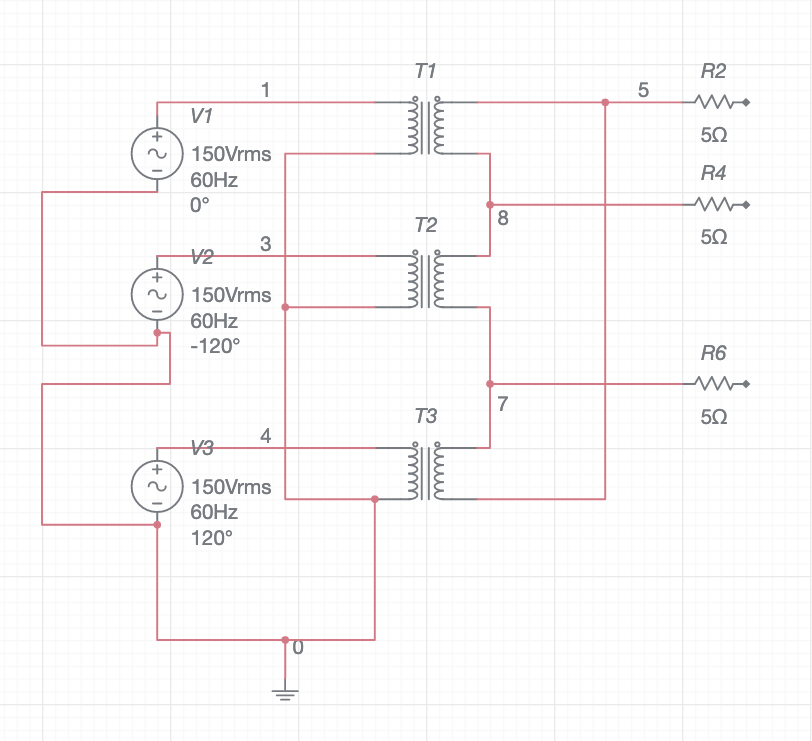
\includegraphics[width=.8\linewidth]{images/output/ydel.png}
    \caption{Circuit diagrams for Y-$\Delta$ three transformer connection.}
    \label{fig:fig}
\end{figure}
\vspace{\fill}

\section{Tools Used}
\begin{itemize}
    \item Three Phase Induction Motor, (220/440V, 9.1/4.55A)
    \item Ammeter (0A - 5A)
    \item Voltmeter (0V - 450V)
    \item Wattmeter
    \item Three Phase AC supply (220V)
    \item Three phase Variac (0-250V)
    \item Connecting wires
\end{itemize}

\section{Data \& Calculation}
\subsection{Data Table:}
\begin{table}[H]
    \centering
    \caption{Blocked Rotor Test}
    \begin{tabular}{|c|c|c|c|c|}
        \hline
        \bf{V\textsubscript{s}} & \bf{I\textsubscript{s}} & \bf{W\textsubscript{1}} & \bf{W\textsubscript{2}} & \bf{W\textsubscript{T}} \\
        \hline
        105                     & 2.28                    & 500                     & 260                     & 760                     \\
        \hline
    \end{tabular}
\end{table}
\begin{table}[H]
    \centering
    \caption{No Load Test}
    \begin{tabular}{|c|c|c|c|c|}
        \hline
        \bf{V\textsubscript{0}} & \bf{I\textsubscript{0}} & \bf{W\textsubscript{1}} & \bf{W\textsubscript{2}} & \bf{W\textsubscript{T}} \\
        \hline
        438                     & 2.4                     & 860                     & 140                     & 720                     \\
        \hline
    \end{tabular}
\end{table}

\subsection{Calculation:}
\subsubsection*{Blocked rotor test:}
Total resistance of the motor as referred to primary,\\\\
\(R_{01} = \frac{V_s^2}{W_T} = \frac{105^2}{760}=14.5\)\\\\
Total impedance of the motor as referred to primary,\\\\
\(Z_{01} = \frac{V_0}{\sqrt{3}\times I_s} = \frac{105}{\sqrt{3} \times 2.28}=26.58\)\\\\
Total leakage reactance of the motor as referred to primary,\\\\
\(X_{01} = \sqrt{Z_{01}^2 - R_{01}^2} = \sqrt{26.58^2 - 14.5^2}= 22.27\)

\subsubsection*{No-load test:}
\(R_{0} = \frac{W_T}{I_0^2} = \frac{720}{2.4^2}=125\)\\\\
Total impedance of the motor as referred to primary,\\\\
\(Z_{01} = \frac{V_0}{I_0} = \frac{438}{2.4} = 182.5\)\\\\
\(X_{0} = \sqrt{Z_0^2 - R_0^2} = \sqrt{182.5^2 - 125^2}= 132.97\)
\\\\
The rated voltage and current of the tested induction motor are 440V and 4.55 A respectively. So If it is assumed that at rated condition p.f is 0.80, then the input power is \(\sqrt{3}V_LI_L cos\theta = 2774.05 W\)\\\\
And Losses\\\\
\(= P_{CU}+P_{CORE} + P_{F+W} =1001.5 W\)\\\\
\% Efficiency \(=( Output/ input)\times100\%\)\\\\
\% Efficiency \( = \frac{(Input- Losses) \times100}{Input} \% = 63.9 \%\)\\\\
Efficiency \(= Output/ (Output + losses)= 63.9\%\)


\section{Discussion}
Small motor efficiency can be assessed by immediately loading them and measuring the input and output powers. However, it is impossible to arrange so much load for huge motors. If we directly test the load, the power loss will be significant. As a result, the no load and blocked rotor tests are performed to measure the efficiency of a three-phase induction motor. During the experiment, an issue developed when the wattmeter caught fire due to a flaw in the connections.


\section{Conclusion}
Since this experiment was done with AC supply, utmost caution was exercised to avoid any accident. Additionally, for the no load test, the current wasn't increased to rated current as voltage is high and it was dangerous with the available equipment. To avoid any dangers, the experiment was done within the supervision of experienced personnel.

\bibliographystyle{IEEEtran}
\bibliography{ref}

\end{document}